%%%%%%%%%%%%%%%%%%%%%%%%%%%%%%%
%   Figures for chapter 2
%%%%%%%%%%%%%%%%%%%%%%%%%%%%%%%

\newcommand{\figrlloop}{
    \begin{figure}
        \centering
        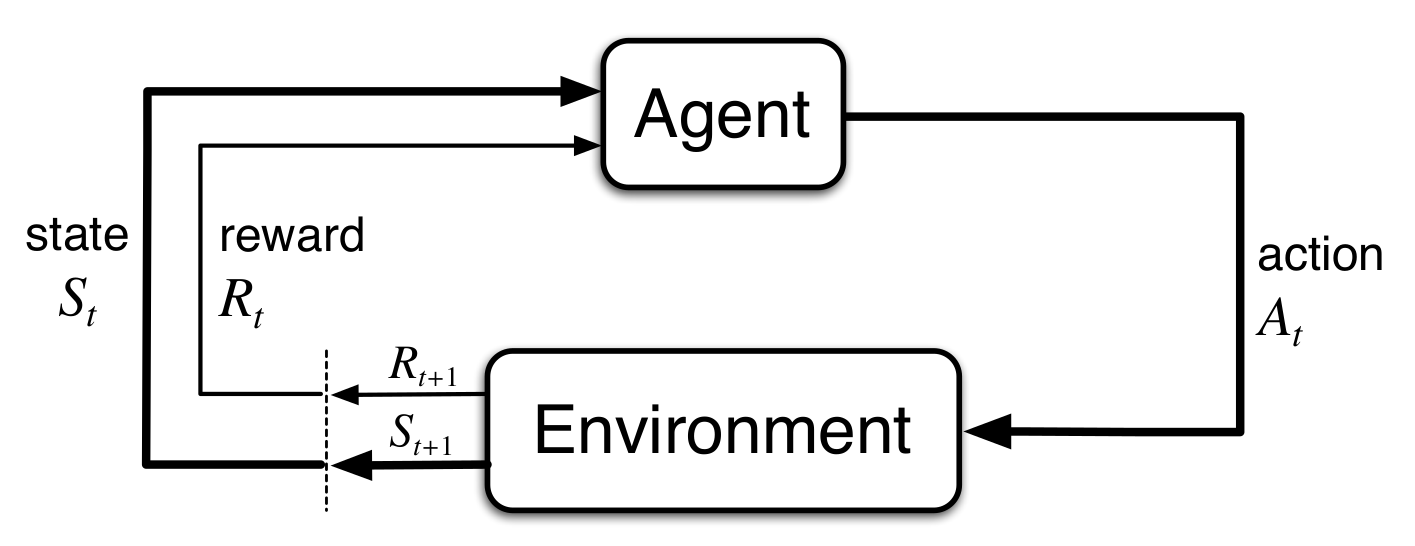
\includegraphics[width=5in]{./chapters/chapter_2/imgs/img_rl_loop.png}
        \caption{Agent-Environment interaction loop}
        \label{fig:ch2_rlloop}
    \end{figure}
}

\newcommand{\figdrlsamplesFirst}{
    \begin{figure}
        \centering
        \begin{subfigure}[b]{0.4\textwidth}
            \centering
            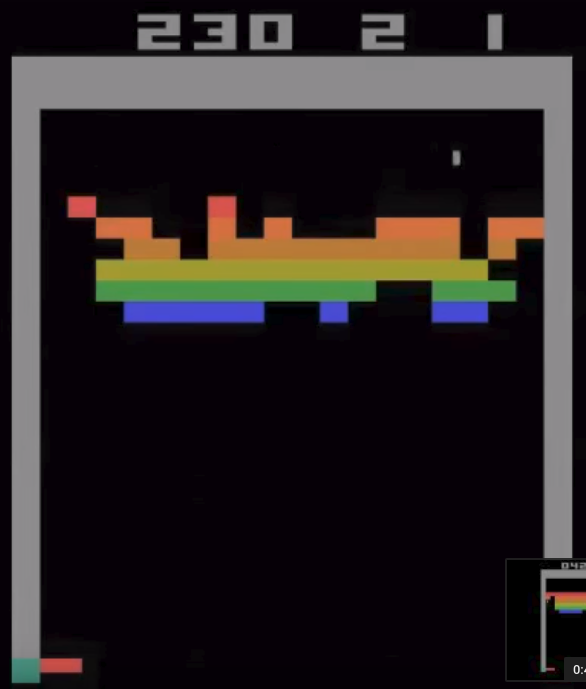
\includegraphics[width=0.9\textwidth]{./chapters/chapter_2/imgs/img_dqn_breakout.png}
            \caption{}
            \label{fig:ch2_dqn_breakout}
        \end{subfigure}
        \begin{subfigure}[b]{0.4\textwidth}
            \centering
            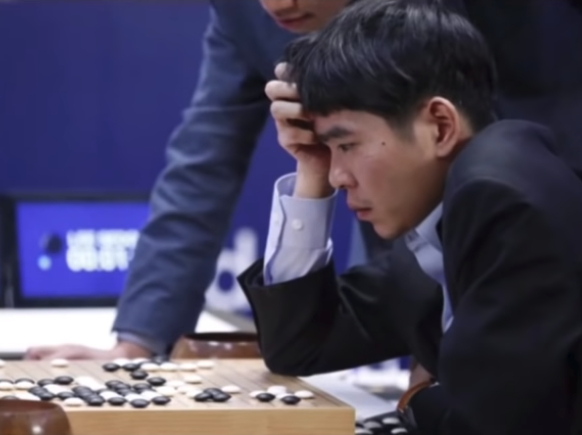
\includegraphics[width=0.9\textwidth]{./chapters/chapter_2/imgs/img_alphago.png}
            \caption{}
            \label{fig:ch2_alphago}
        \end{subfigure}
        \caption{Some DeepRL success stories: (a) DQN agent playing atari breakout \citep{DQNAtari},
                                              (b) AlphaGo playing against Go champion Lee Sedol \citep{AlphaGo}}
        \label{fig:ch2_drl_stories_1}
    \end{figure}
}

\newcommand{\figdrlsamplesSecond}{
    \begin{figure}
        \centering
        \begin{subfigure}[b]{0.3\textwidth}
            \centering
            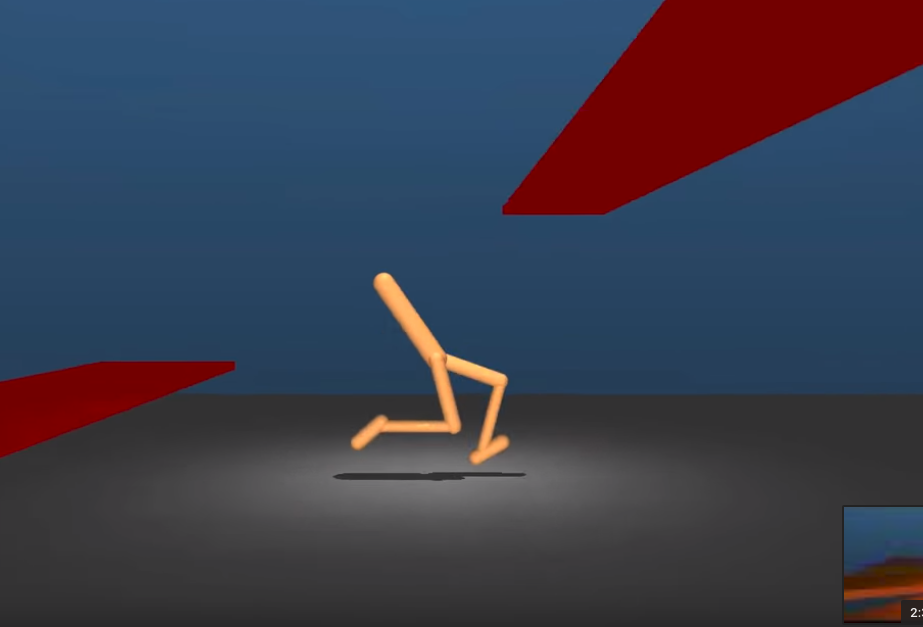
\includegraphics[width=0.9\textwidth]{./chapters/chapter_2/imgs/img_emergence_of_locomotion.png}
            \caption{}
            \label{fig:ch2_emergence_of_locomotion}
        \end{subfigure}
        \begin{subfigure}[b]{0.3\textwidth}
            \centering
            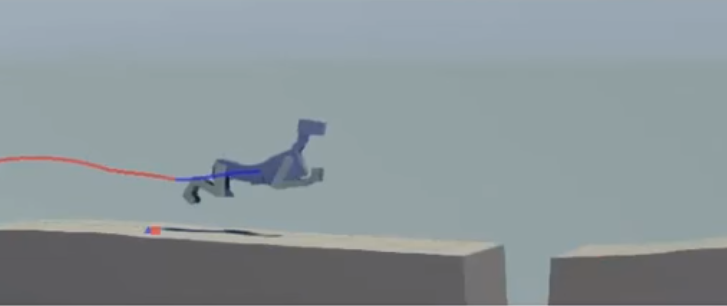
\includegraphics[width=0.9\textwidth]{./chapters/chapter_2/imgs/img_deepterrainrl.png}
            \caption{}
            \label{fig:ch2_deepterrainrl}
        \end{subfigure}
        \begin{subfigure}[b]{0.3\textwidth}
            \centering
            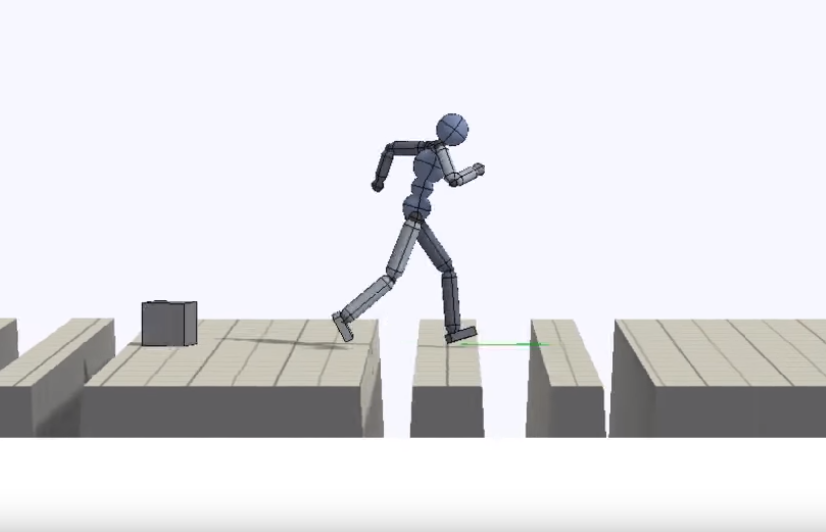
\includegraphics[width=0.9\textwidth]{./chapters/chapter_2/imgs/img_deepmimic.png}
            \caption{}
            \label{fig:ch2_deepmimic}
        \end{subfigure}
        \caption{Some DeepRL success stories: (a) Deepmind's agent running in a simulated environment \citep{DeepmindEmergenceLocomotion},
                                              (b) Simulated dog running in a course with obstacles \citep{DeepTerrainRL},
                                              (c) Simulated character running in an obstacle course, while 
                                                  mimicking humans' natural motion \citep{DeepMimic}}
        \label{fig:ch2_drl_stories_2}
    \end{figure}
}

\newcommand{\figdrlsamplesThird}{
    \begin{figure}
        \centering
        \begin{subfigure}[b]{0.3\textwidth}
            \centering
            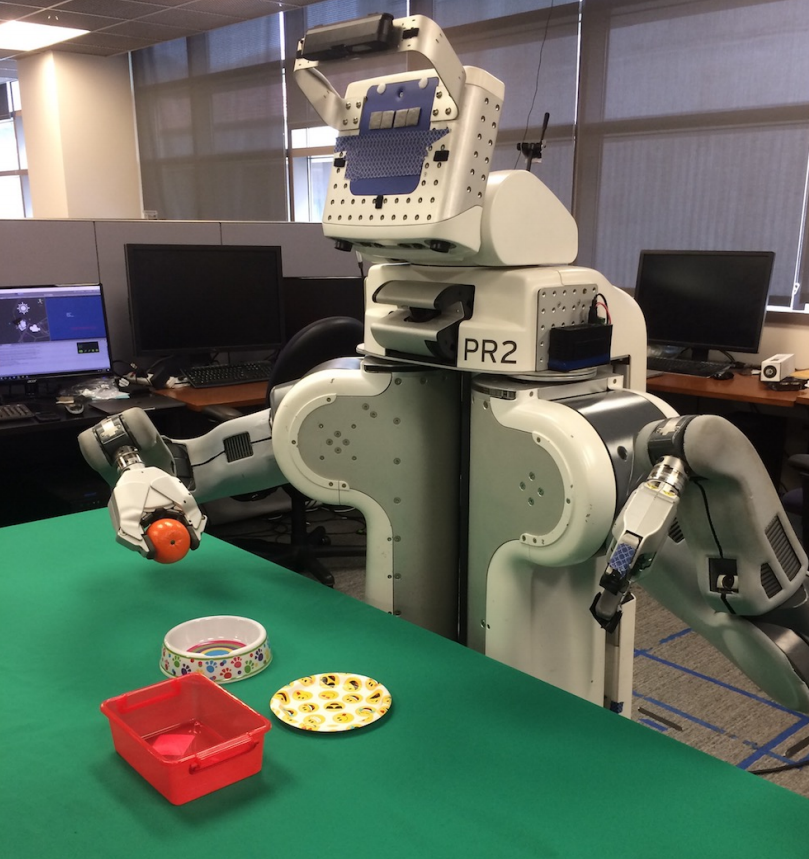
\includegraphics[width=0.9\textwidth]{./chapters/chapter_2/imgs/img_visual_motor_control.png}
            \caption{}
            \label{fig:ch2_visual_motor_control}
        \end{subfigure}
        \begin{subfigure}[b]{0.3\textwidth}
            \centering
            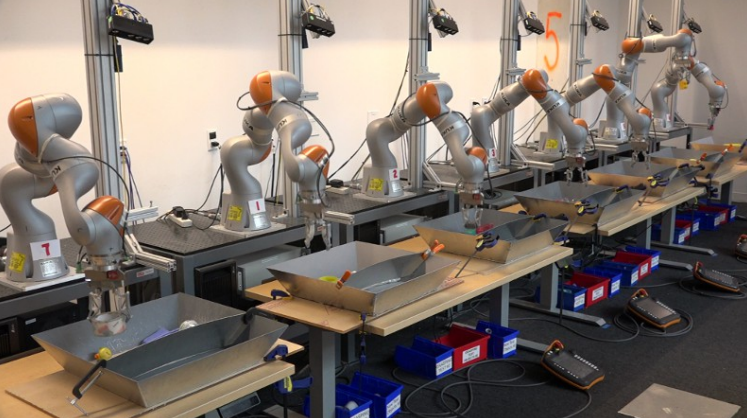
\includegraphics[width=0.9\textwidth]{./chapters/chapter_2/imgs/img_vision_based_robotics.png}
            \caption{}
            \label{fig:ch2_vision_based_robotics}
        \end{subfigure}
        \begin{subfigure}[b]{0.3\textwidth}
            \centering
            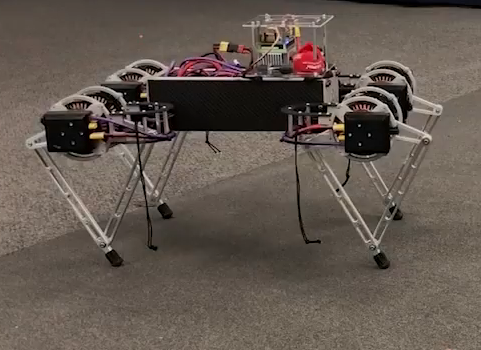
\includegraphics[width=0.9\textwidth]{./chapters/chapter_2/imgs/img_sim_2_real.png}
            \caption{}
            \label{fig:ch2_sim_2_real}
        \end{subfigure}
        \caption{Some DeepRL success stories: (a) PR2 robot learning manipulation tasks \citep{EndToEndVisuoMotorPolicies},
                                              (b) Learning more manipulation tasks using lots of robots \citep{ScalableDeepRL},
                                              (c) Quadruped running in the real world \citep{GoogleBrainSim2Real}}
        \label{fig:ch2_drl_stories_3}
    \end{figure}
}

\newcommand{\figMdpSamples}{
    \begin{figure}
        \centering
        \begin{subfigure}[b]{0.9\textwidth}
            \centering
            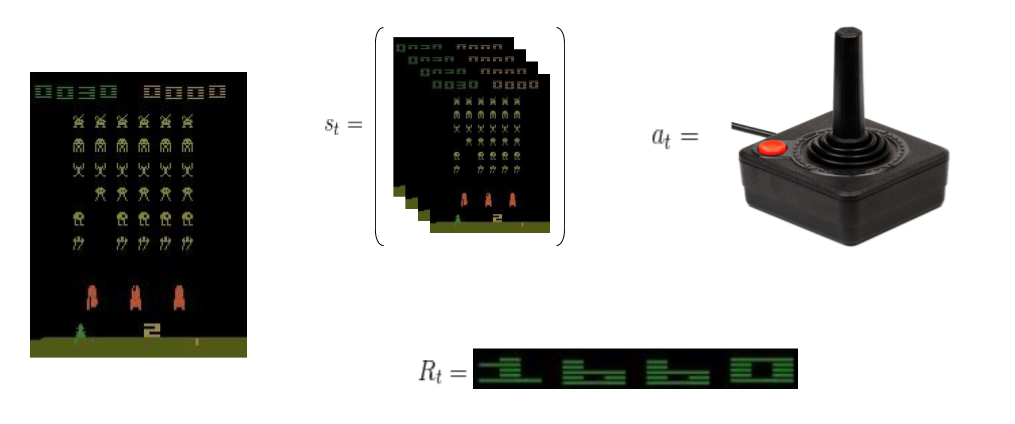
\includegraphics[width=0.9\textwidth]{./chapters/chapter_2/imgs/img_rl_mdp_atari.png}
            \caption{}
            \label{fig:ch2_mdp_sample_atari}
        \end{subfigure}

        \centering
        \begin{subfigure}[b]{0.9\textwidth}
            \centering
            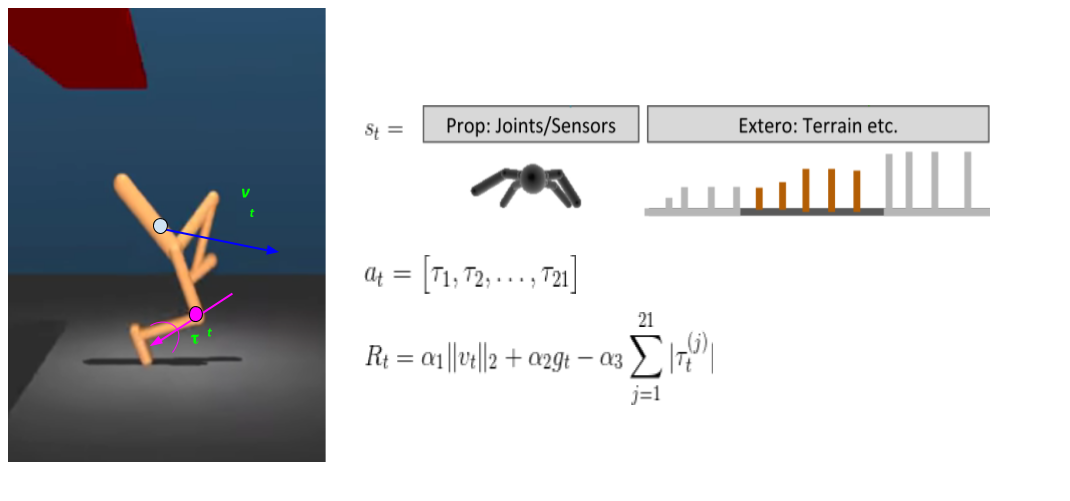
\includegraphics[width=0.9\textwidth]{./chapters/chapter_2/imgs/img_rl_mdp_locomotion.png}
            \caption{}
            \label{fig:ch2_mdp_sample_locomotion}
        \end{subfigure}
        \caption{Some examples of MDPs: (a) MDP modelling an Atari game. 
                                        (b) MDP modelling a locomotion task.}
        \label{fig:ch2_mdps_samples}
    \end{figure}
}

\newcommand{\figRlPolicies}{
    \begin{figure}
        \centering
        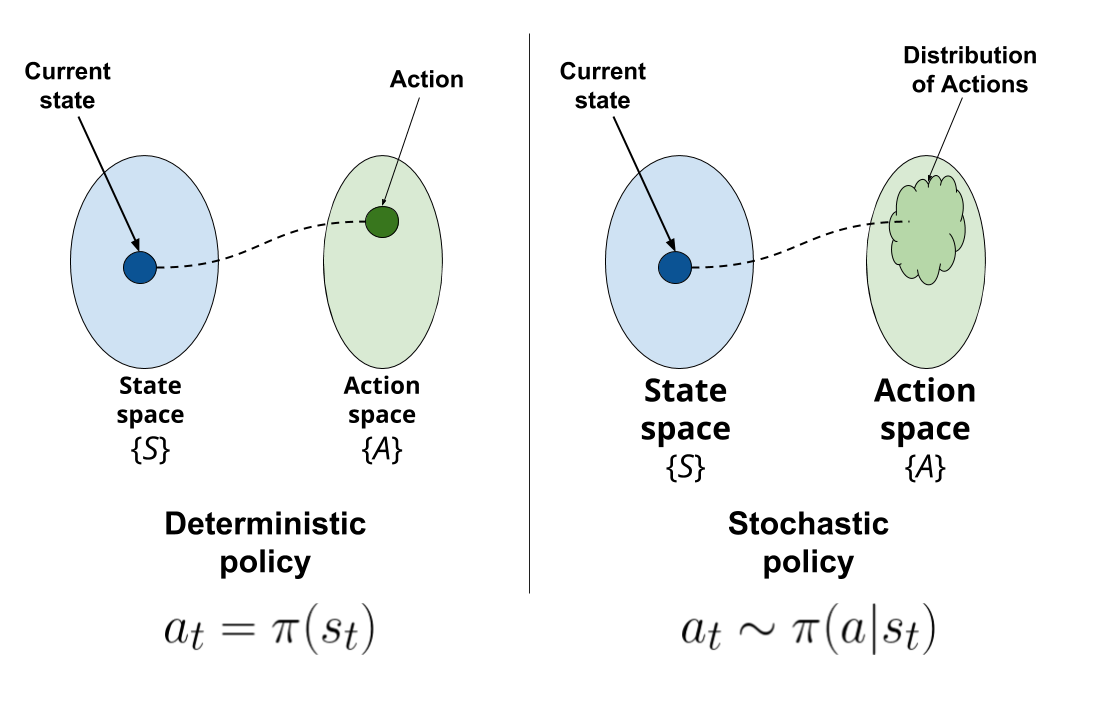
\includegraphics[width=0.9\textwidth]{./chapters/chapter_2/imgs/img_rl_policies.png}
        \caption{Differences between deterministic and stochastic policies.}
        \label{fig:ch2_rl_policies_differences}
    \end{figure}
}

\newcommand{\figRlMethodsLandspace}{
    \begin{figure}
        \centering
        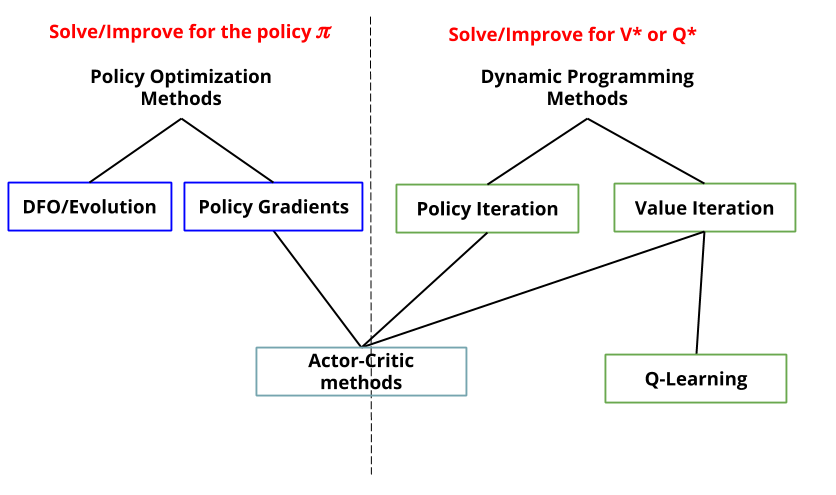
\includegraphics[width=0.9\textwidth]{./chapters/chapter_2/imgs/img_rl_methods.png}
        \caption{RL solution methods landspace. \textbf{Value-based methods} (right) solve for the policy 
                 indirectly, whereas \textbf{Policy-based methods} (left) solve for the policy directly.}
        \label{fig:ch2_rl_policies_differences}
    \end{figure}
}

\newcommand{\figRlPolicyGradientsIntuition}{
    \begin{figure}[!b]
        \centering
        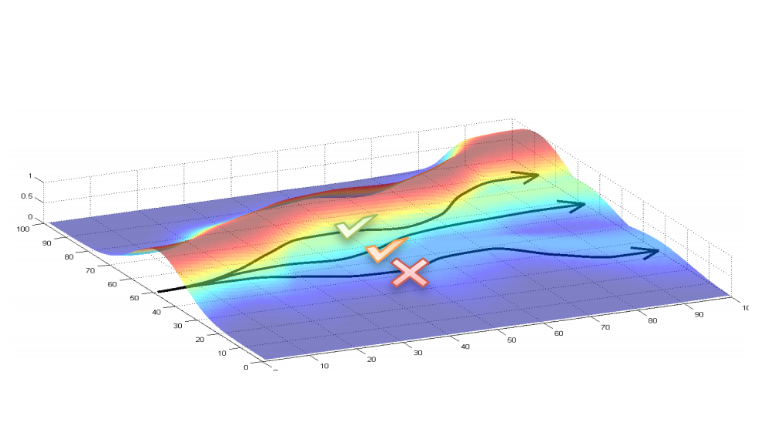
\includegraphics[width=0.8\textwidth]{./chapters/chapter_2/imgs/img_rl_pg_intuition.png}
        \caption{Intuition behind Policy Gradients. Actions that yield good trajectories are encouraged}
        \label{fig:ch2_rl_pg_intuition}
    \end{figure}
}

\newcommand{\figRlPolicyParametrization}{
    \begin{figure}
        \centering
        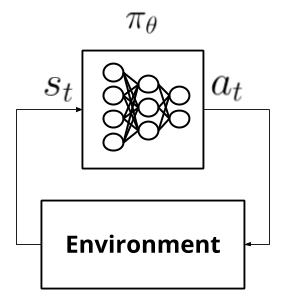
\includegraphics[width=0.225\textwidth]{./chapters/chapter_2/imgs/img_policy_parametrization.png}
        \caption{Parameterization of a policy $\pi$ using a Neural Network}
        \label{fig:ch2_rl_policy_parametrization}
    \end{figure}
}

\newcommand{\figALEgames}{
    \begin{figure}[H]
        \centering
        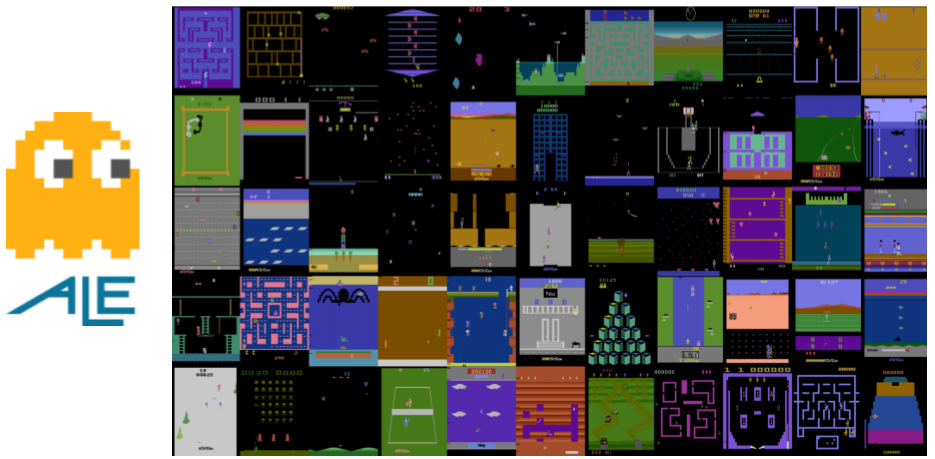
\includegraphics[width=0.6\textwidth]{./chapters/chapter_2/imgs/img_atari_learning_environment.png}
        \caption{Games in the Atari Learning Environment.}
        \label{fig:ch2_ale_games}
    \end{figure}
}

\newcommand{\figOpenAIEnvs}{
    \begin{figure}[H]
        \centering
        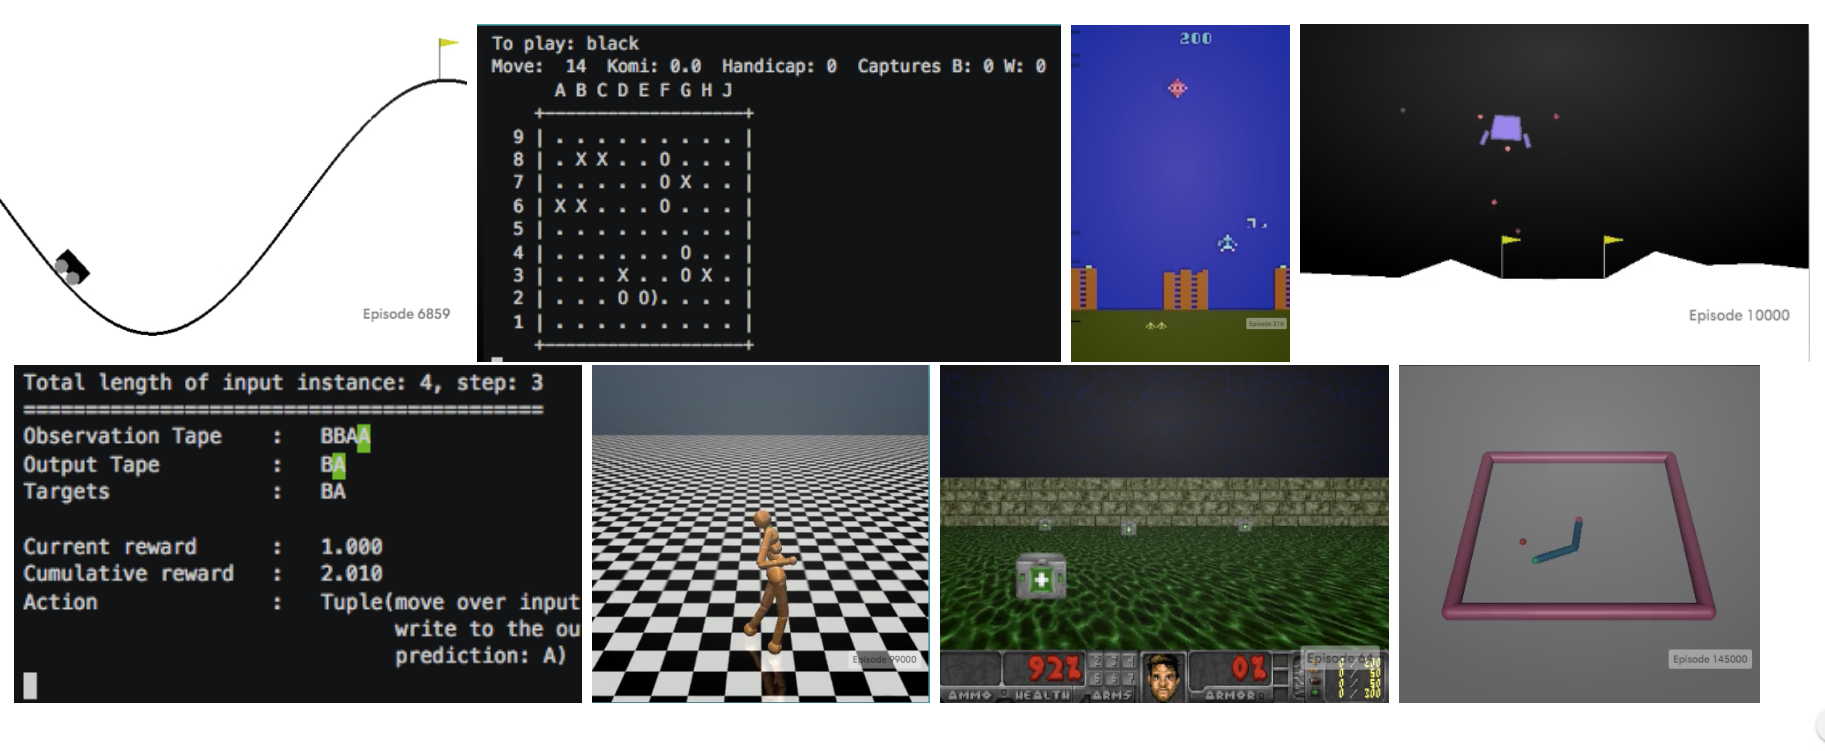
\includegraphics[width=0.9\textwidth]{./chapters/chapter_2/imgs/img_openai_gym_envs.png}
        \caption{Environments in OpenAI Gym.}
        \label{fig:ch2_gym_envs}
    \end{figure}
}

\newcommand{\figDeepmindLabEnvs}{
    \begin{figure}[H]
        \centering
        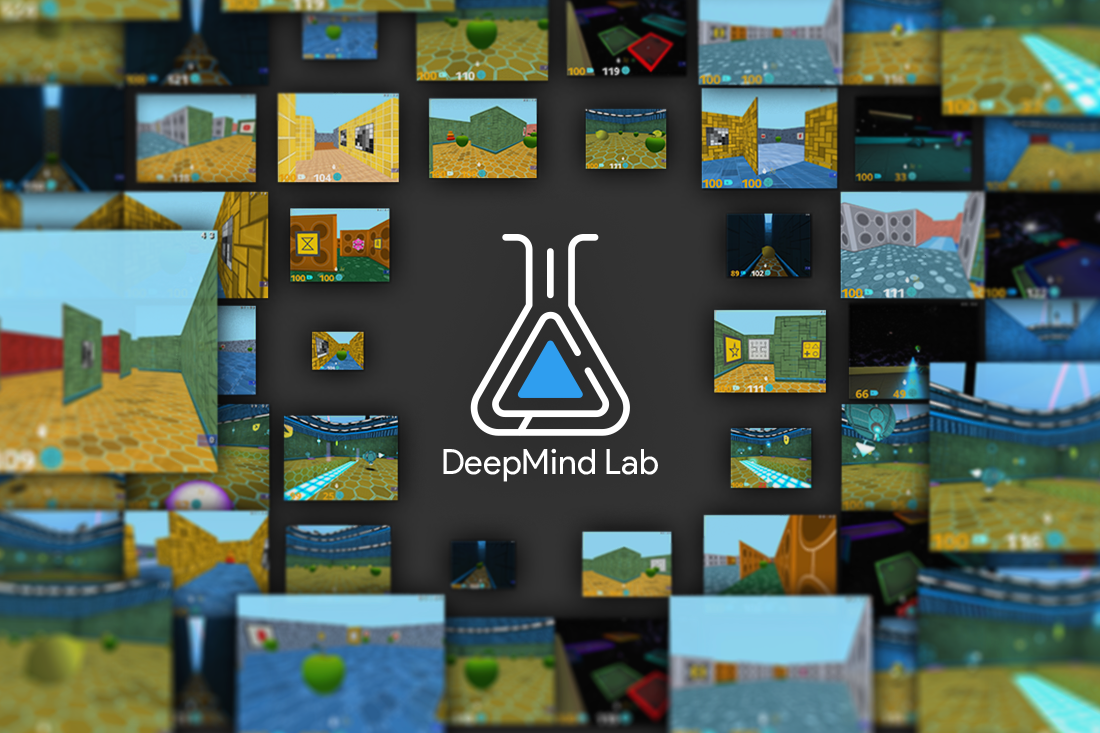
\includegraphics[width=0.9\textwidth]{./chapters/chapter_2/imgs/img_deepmind_lab.png}
        \caption{Environments in Deepmind Lab}
        \label{fig:ch2_deepmind_lab}
    \end{figure}
}

\newcommand{\figPhysicsEngineLoop}{
    \begin{figure}
        \centering
        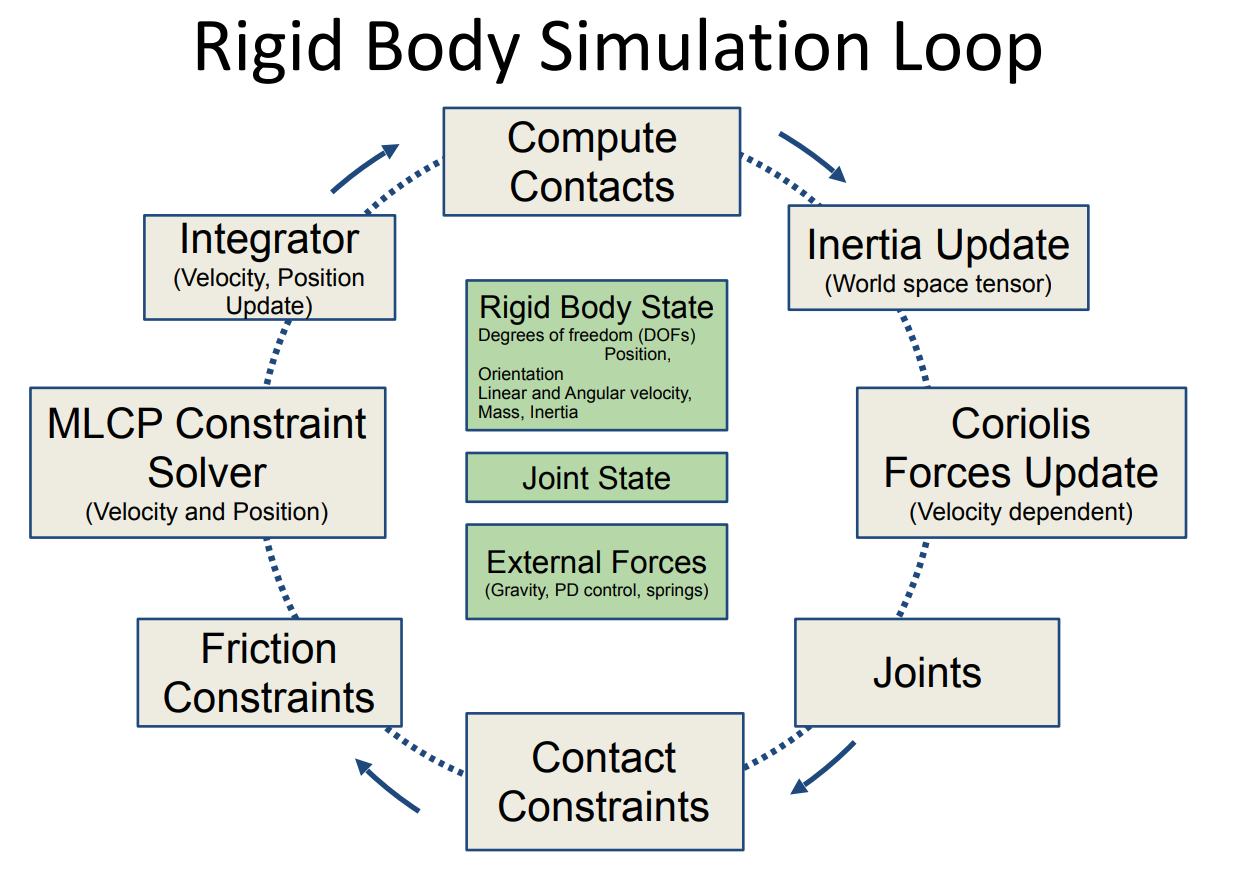
\includegraphics[width=0.6\textwidth]{./chapters/chapter_2/imgs/img_physics_engine_loop.png}
        \caption{A common pipeline used by physics engines, from \citep{ErwinCowmansMlcp}}
        \label{fig:ch2_physics_engines_loop}
    \end{figure}
}

\newcommand{\figKinTreeRepresentation}{
    \begin{figure}
        \centering
        \begin{subfigure}[b]{0.45\textwidth}
            \centering
            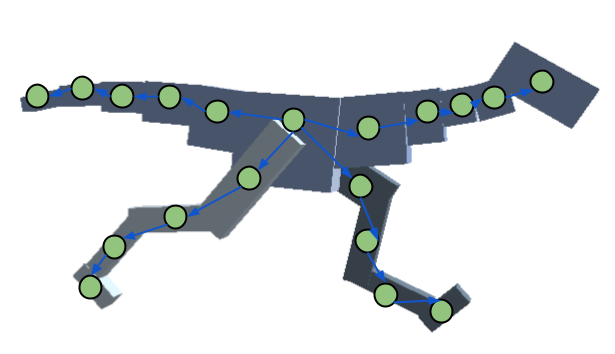
\includegraphics[width=0.9\textwidth]{./chapters/chapter_2/imgs/img_dyno_agent.png}
            \caption{}
            \label{fig:ch2_dyno_agent}
        \end{subfigure}
        \begin{subfigure}[b]{0.45\textwidth}
            \centering
            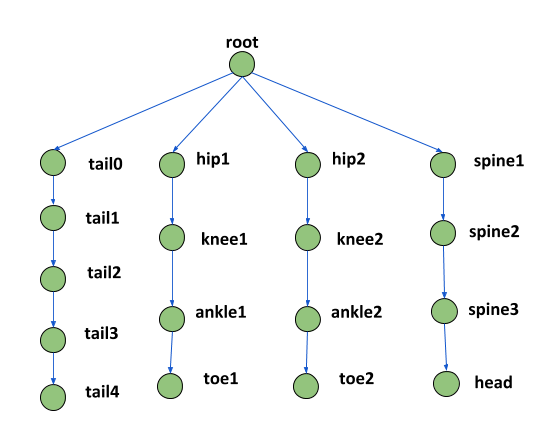
\includegraphics[width=0.9\textwidth]{./chapters/chapter_2/imgs/img_kinematic_tree.png}
            \caption{}
            \label{fig:ch2_kintree}
        \end{subfigure}
        \caption{An agent for a locomotion task. a) The agent with its bodies tagged. 
                                                 b) A kinematic tree representing that agent}
        \label{fig:ch2_kinematic_tree_representation}
    \end{figure}
}

\newcommand{\figActuationModels}{
    \begin{figure}
        \centering
        \begin{subfigure}[b]{0.45\textwidth}
            \centering
            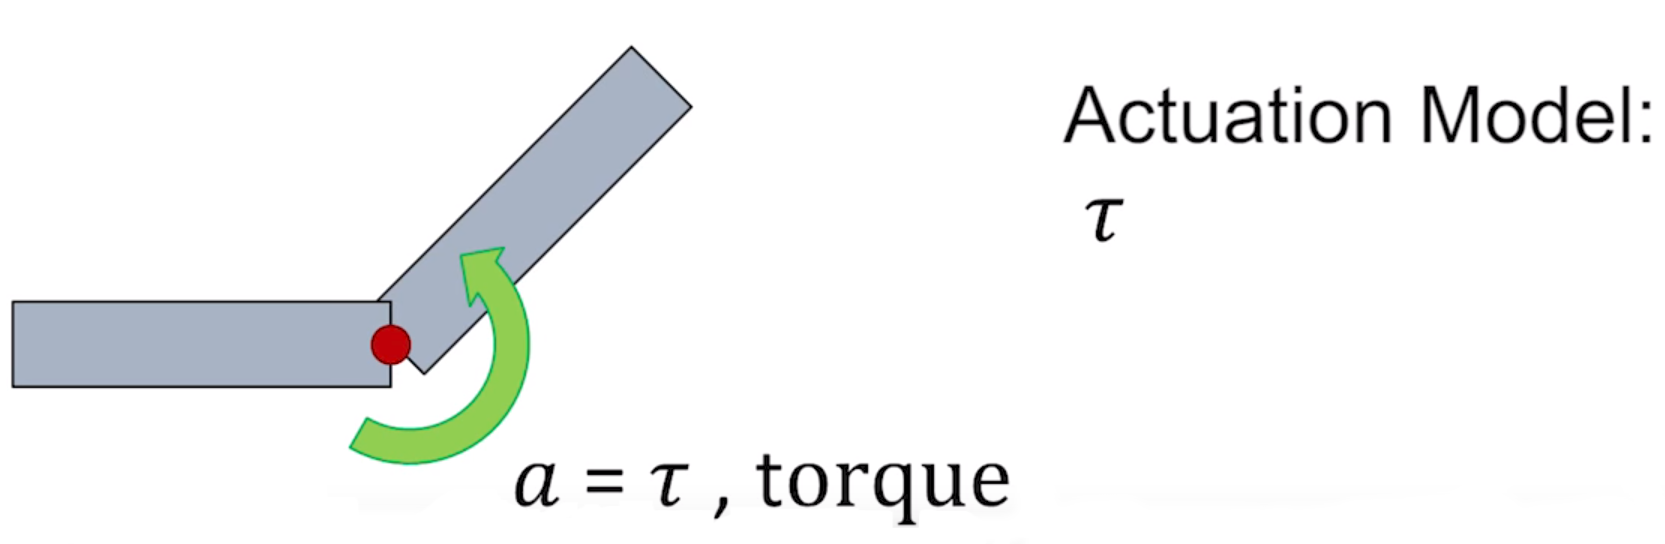
\includegraphics[width=0.8\textwidth]{./chapters/chapter_2/imgs/img_actuation_torque.png}
            \caption{}
            \label{fig:ch2_actuation_torques}
        \end{subfigure}
        \begin{subfigure}[b]{0.45\textwidth}
            \centering
            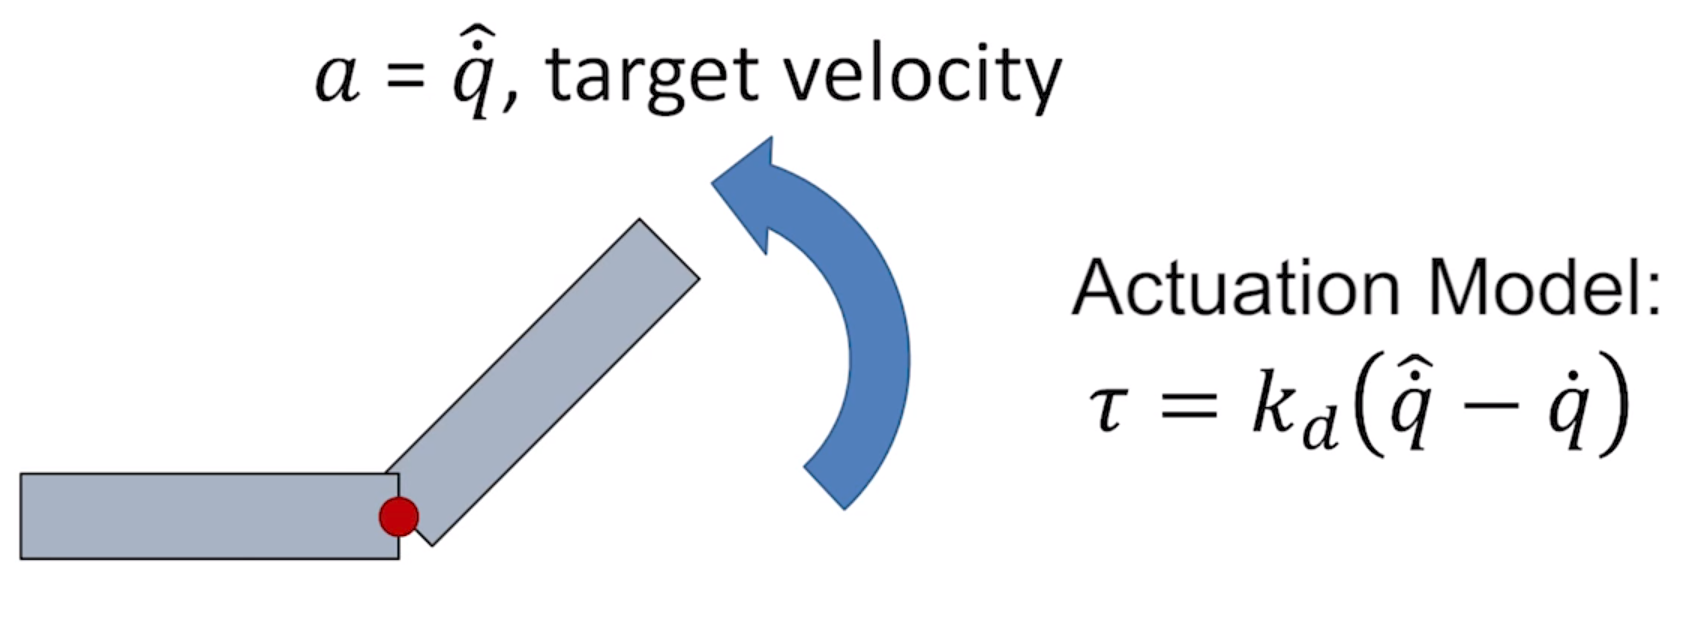
\includegraphics[width=0.8\textwidth]{./chapters/chapter_2/imgs/img_actuation_target_velocities.png}
            \caption{}
            \label{fig:ch2_actuation_target_velocities}
        \end{subfigure}

        \centering
        \begin{subfigure}[b]{0.45\textwidth}
            \centering
            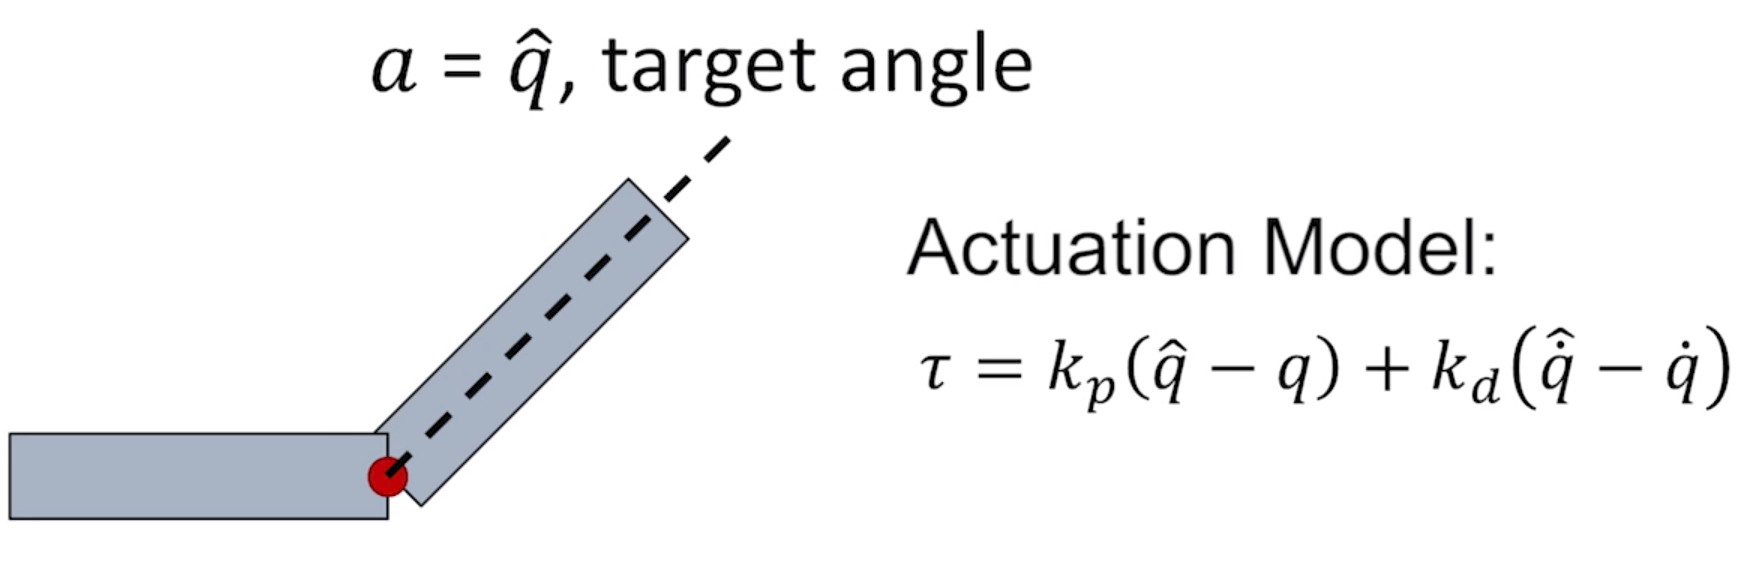
\includegraphics[width=0.8\textwidth]{./chapters/chapter_2/imgs/img_actuation_target_angles.png}
            \caption{}
            \label{fig:ch2_actuation_target_angles}
        \end{subfigure}
        \begin{subfigure}[b]{0.45\textwidth}
            \centering
            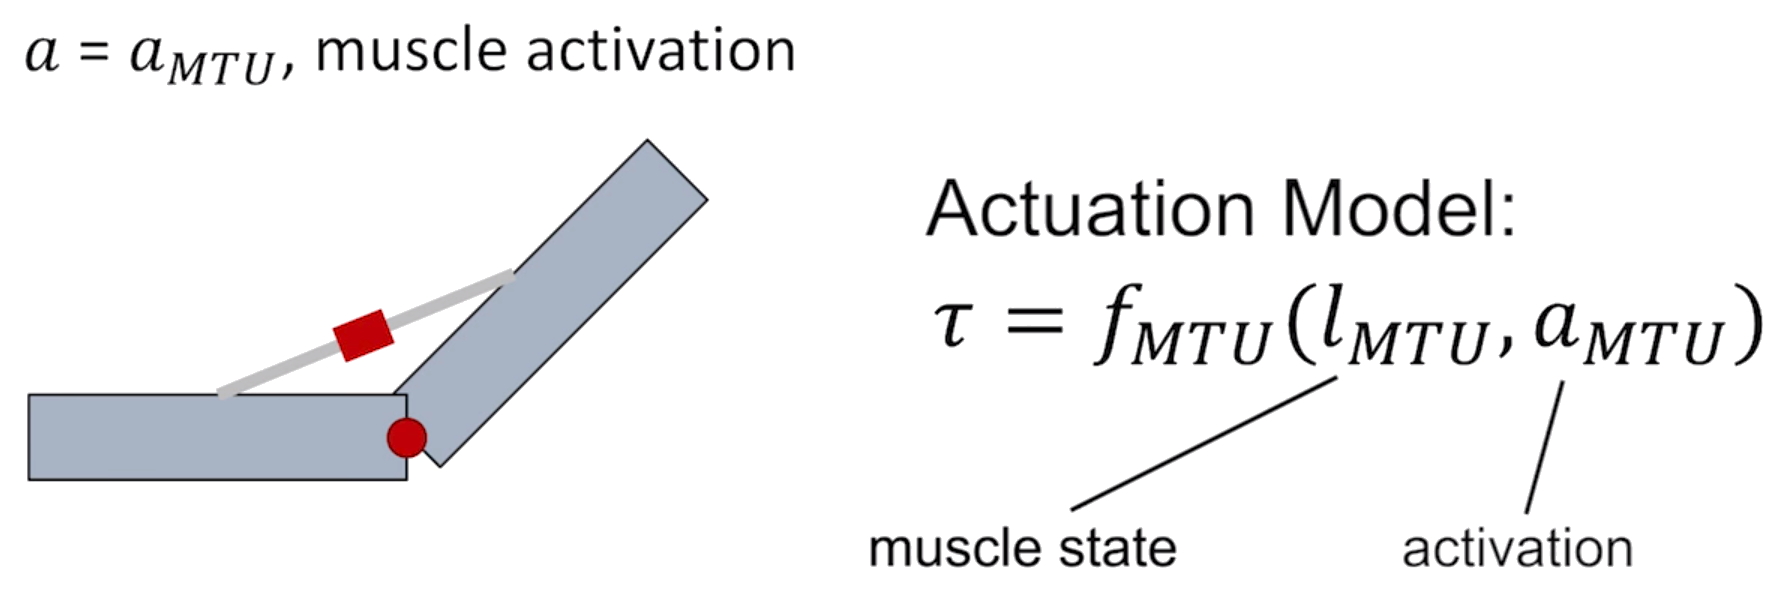
\includegraphics[width=0.8\textwidth]{./chapters/chapter_2/imgs/img_actuation_muscle_activation.png}
            \caption{}
            \label{fig:ch2_actuation_muscle_activations}
        \end{subfigure}
        \caption{An agent for a locomotion task. a) The agent with its bodies tagged. 
                                                 b) A kinematic tree representing that agent}
        \label{fig:ch2_actuation_models}
    \end{figure}
}